\documentclass[/Users/ikedahajime/GitHub/reserch/master_report/thesis]{subfiles}
% このファイル内だけのコマンド
\begin{document}
\chapter{結果}
\section{CABPの結果}
この章では、高密度のCABPを円形領域に閉じ込めた時の結果を示す。%小説での結果のreview
\subsection{系全体のダイナミクス}
まず、時間依存性について議論する。はじめに、規格化された角運動量の時間変化を見る。
\figref{fig:CABP_V_timedep}はパラメータを変化させた時の規格化された角運動量$V$の時間依存性を表すグラフである。
この図におけるパラメータは密度$\varphi=1.209$、$R=10$である。
代表的なパラメータとして(a)は$R_{\Omega}=0.1$、(b)は$R_{\Omega}=10$、(c)は$R_{\Omega}=1000$
を選んだ。3つの図を比較すると、まず$R_{\Omega}$が小さい(a)では$V$の
絶対値が小さく、各粒子がそれぞれ異なる方向へ運動しており、系全体での渦が生じていないことが分かる。
次に$R_{\Omega}$を大きくした(b)では$V$の絶対値は1に近づいており、またその符号は正負に振動している。%???
これは粒子全体が一方向に回転していることを示しており、系全体が渦をなして回転し、その方向は周期的に反転する
ことがわかる。
最後により$R_{\Omega}$を大きくした(c)を見ると、$V$は時間によらず1で一定であり、この領域では粒子全体が1つの渦となって、
定常的な流れをなしていることがわかる。ここでは、(a)のように$V$の絶対値が小さく粒子が一方向に進まない領域を乱雑相、(b)のように$V$の絶対値が
1に近く、その符号が正負に振動している領域を振動相、(c)のように$V$の値が時間によらず1で一定の領域を定流相と呼ぶことにする。\\



\begin{figure}[H]
    \centering
    \begin{tabular}{c}
    % ----- image 1 =====
        \begin{minipage}{0.3\hsize}
            \text{(a)}
            % \centering
            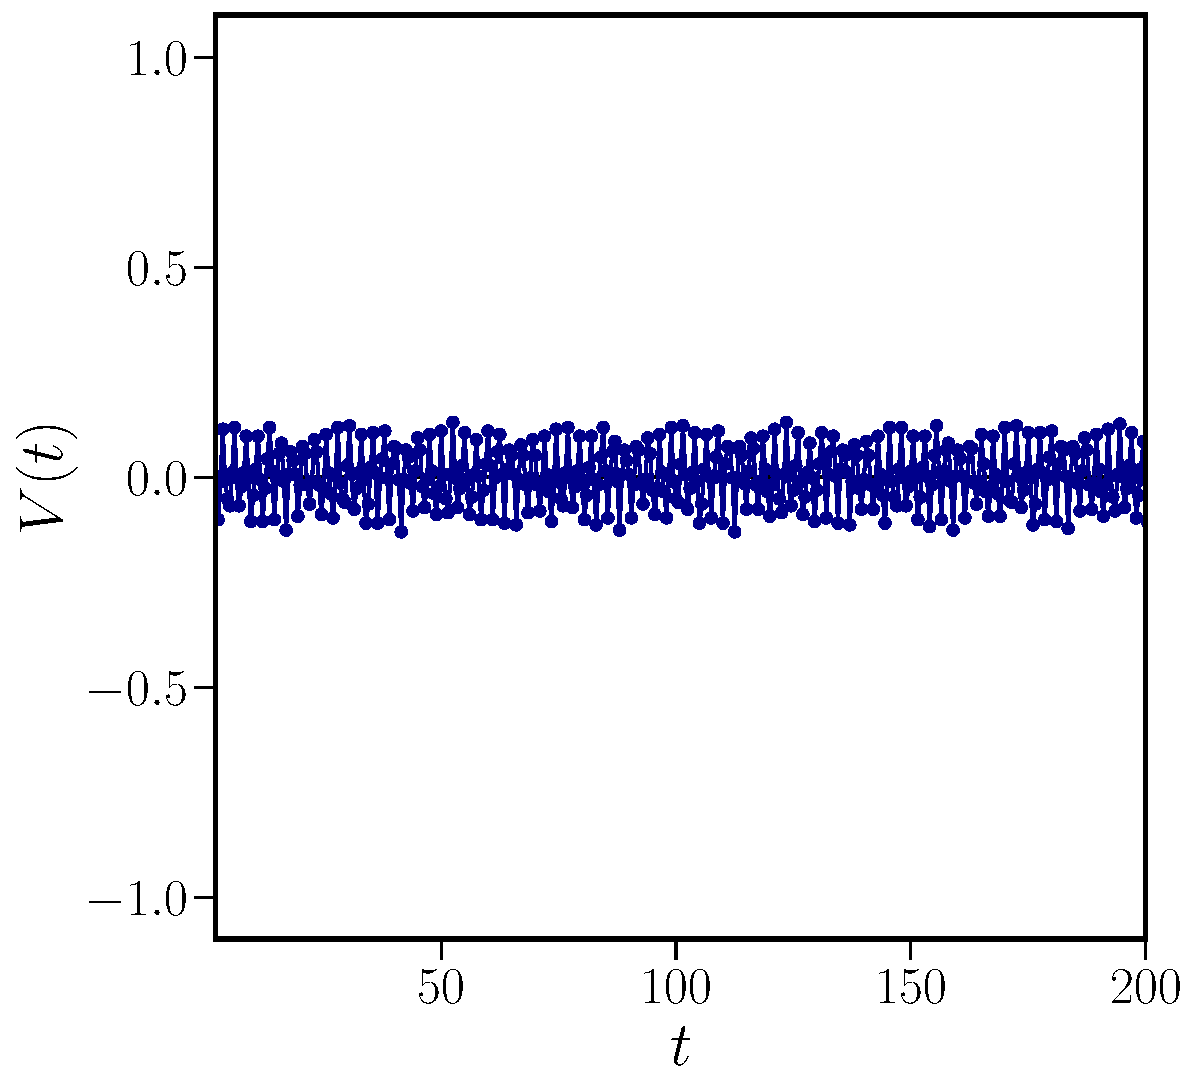
\includegraphics[width=\textwidth]{img/hloabp/figscompANIME/onesR9.963lo1.209Ms0.0ta0Rc0.1Rbit0.0v021.pdf}
        \end{minipage}
    % ----- image 2 =====
        \begin{minipage}{0.3\hsize}
            \text{(b)}
            % \centering
            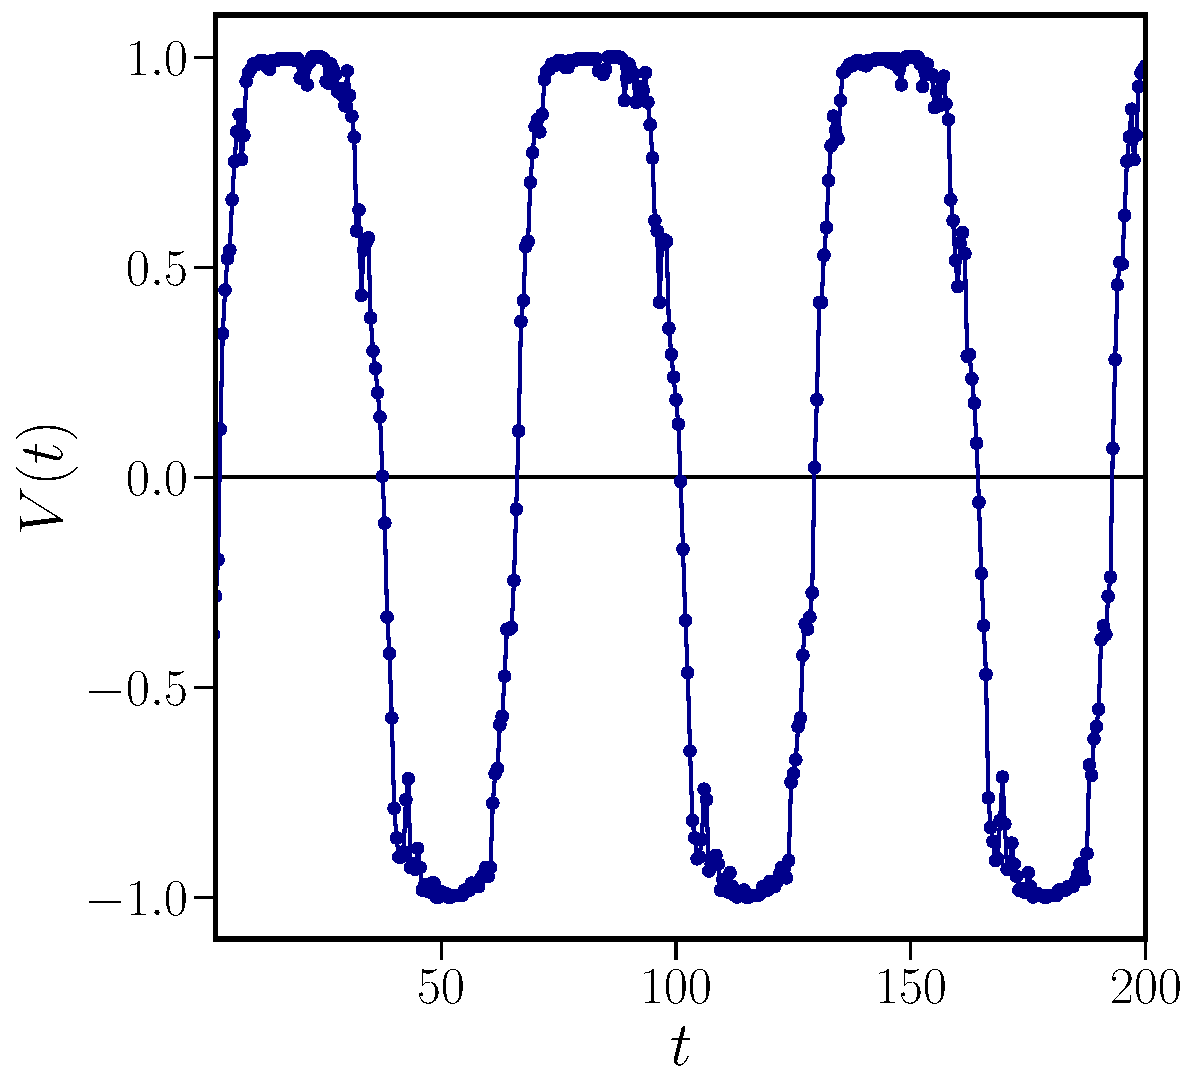
\includegraphics[width=\textwidth]{img/hloabp/figscompANIME/onesR9.963lo1.209Ms0.0ta0Rc10Rbit0.0v021.pdf}
        \end{minipage}
    % ----- image 3 =====
        \begin{minipage}{0.3\hsize}
            \text{(c)}
            % \centering
            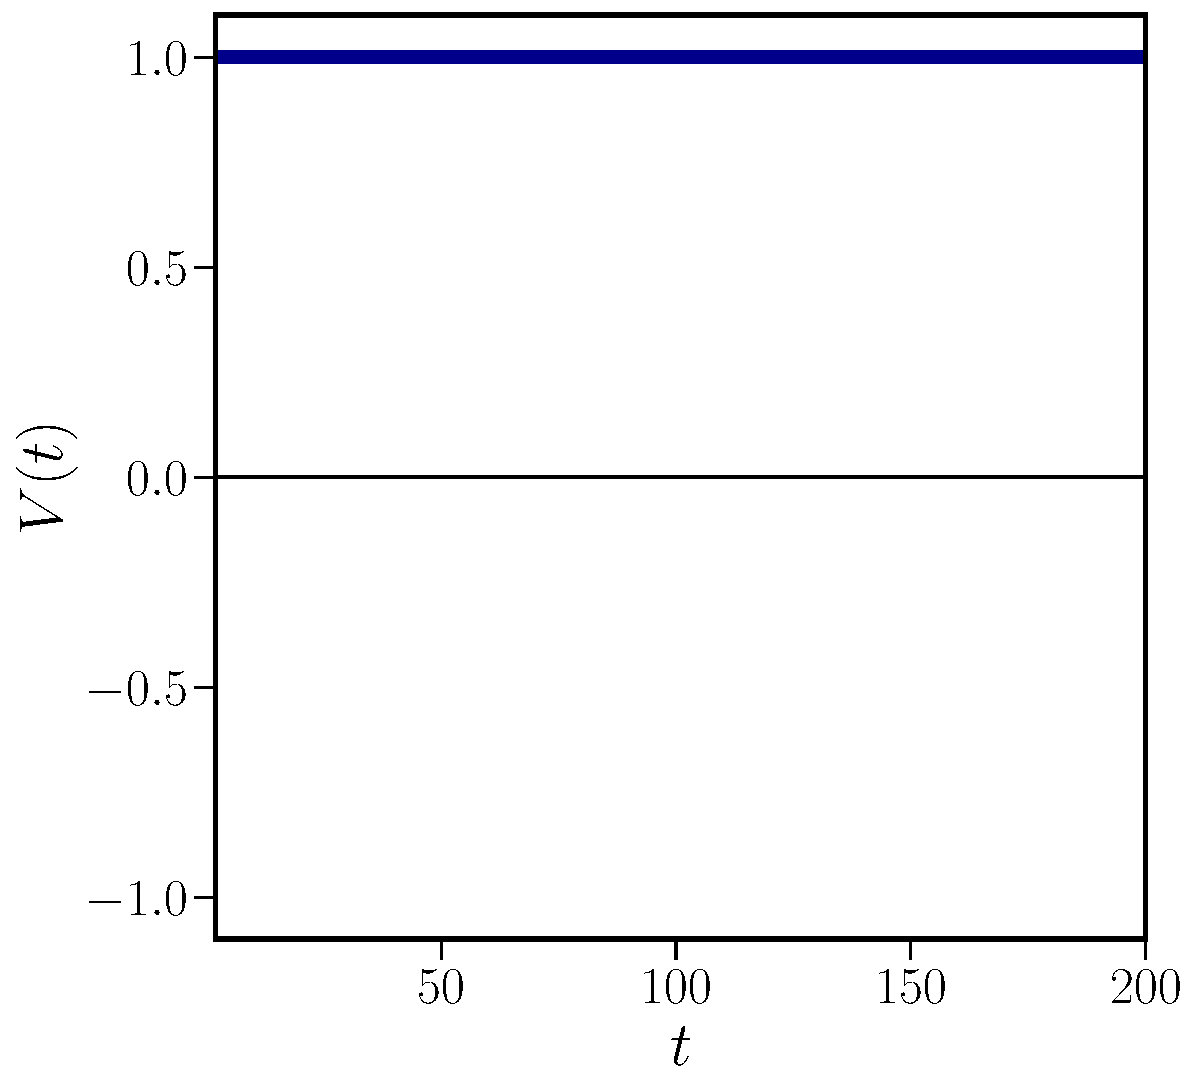
\includegraphics[width=\textwidth]{img/hloabp/figscompANIME/onesR9.963lo1.209Ms0.0ta0Rc1000Rbit0.0v021.pdf}
        \end{minipage}
    \end{tabular}
    \caption[Four sample images]
    {
        円の中に拘束された高密度CABPにおける$V(t)$の時間依存性。(a) $R_{\Omega}=0.1$ (b) $R_{\Omega}=10$ (c) $R_{\Omega}=1000$ で、
        $R=10 , \varphi=1.209$。
        $R_{\Omega}$を大きくするにつれて、振幅が大きくなり、また定常的な流れへと遷移していることがわかる。
    }
    \label{fig:CABP_V_timedep}
\end{figure}

これらの相を定量的に評価するため、$V(t)$の時間平均を考える。\figref{fig:vabs_vave_state}(a)、(c)は$V$の絶対値の平均値、
(b)、(d)は$V$の平均値と$R_\Omega$のグラフである。横軸は$R_{\Omega}$で、横軸のみ対数軸になっている。
いずれも$R_\Omega$を大きくするにつれて大きくなるが、スケールすると(c)、(d)のようになる。
(c)は横軸を$\xi_\bot/R \propto R_\Omega^{1/2}/R$\cite{kurodaLongrangeTranslationalOrder2024}で、
(d)は横軸を$R_\Omega/R$でそれぞれスケールした図である。このようにスケールすると各半径のグラフが重なる。
これは$|V|$の変化、つまり全粒子の整列が$R_\Omega^{1/2}$に、$V$の変化、つまり流れの定常化が$R_\Omega^1$
に比例して起きていることを示す。特に$|V|$の変化、つまり乱雑相と振動相の変化では$R\simeq\xi_\bot$においてパラメータの値が大きくなっている。
バルク系における相関長の大きさが拘束している円の半径と同等になったときに系全体が1つの渦になっていることを
示しており、これは他の系における結果と一致する。\\%TODO*cite
\begin{figure}[htbp]
    \centering
    \begin{tabular}{c}
        \begin{minipage}{0.3\hsize}
            % \centering
            \text{(a)}
            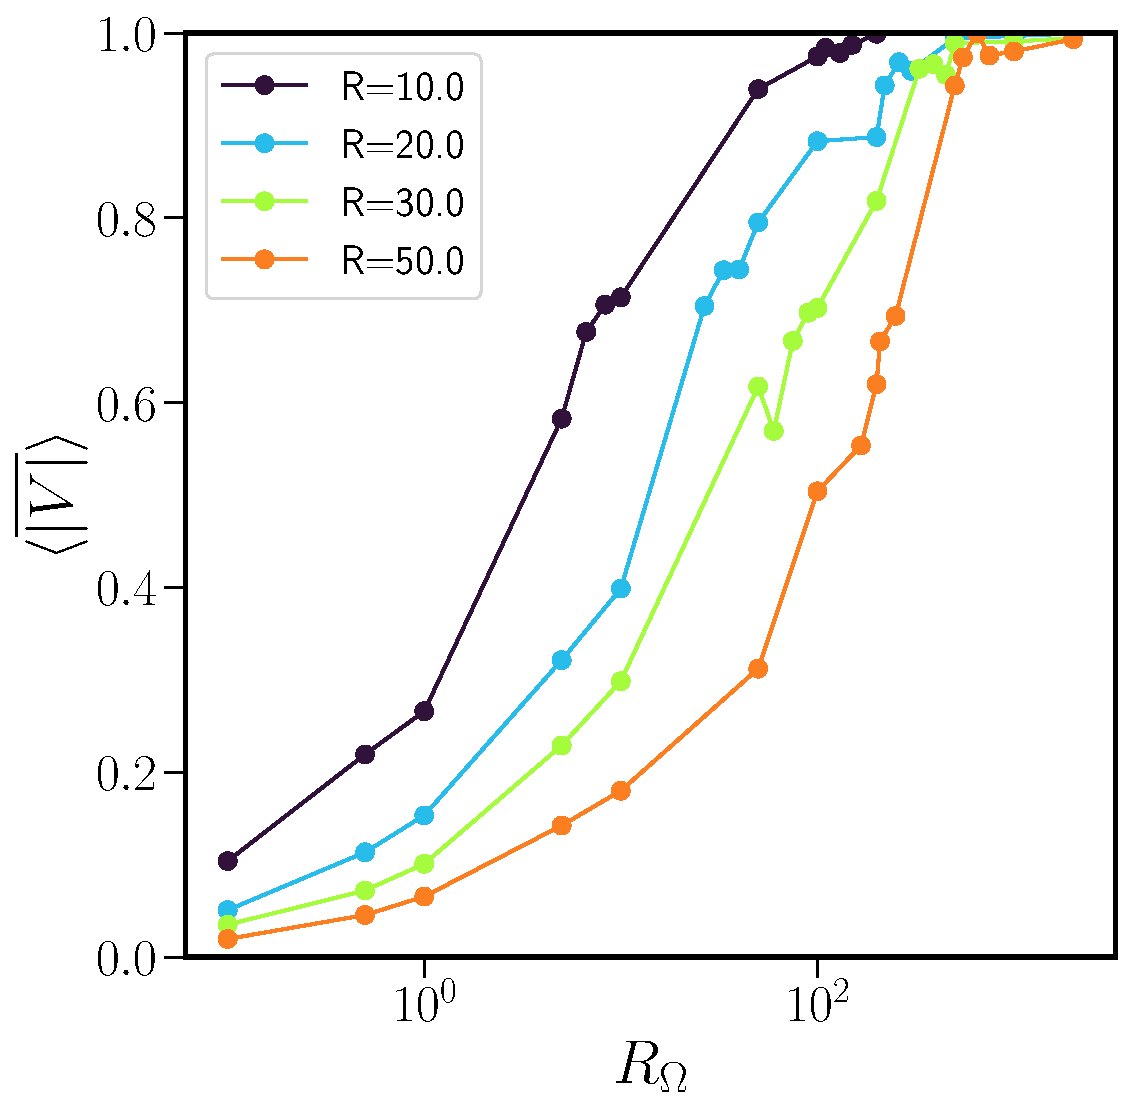
\includegraphics[width=\textwidth]{img/chiral/HAMLOD3_RAT40/abs_vlog_x.pdf}
        \end{minipage}
            \begin{minipage}{0.3\hsize}
                % \centering
                \text{(b)}
                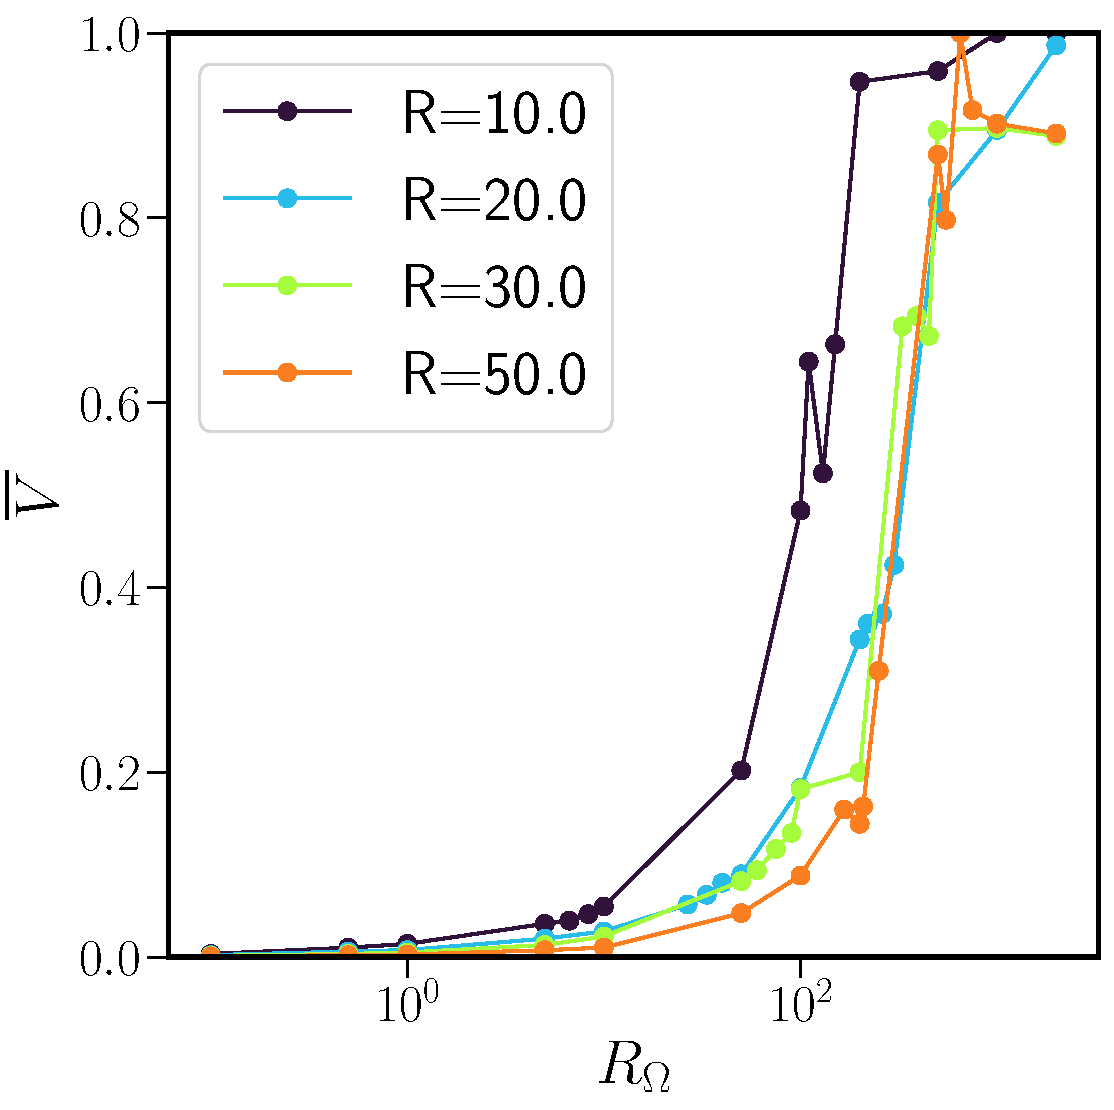
\includegraphics[width=\textwidth]{img/chiral/HAMLOD3_RAT40/sumvlog_x.pdf}
        \end{minipage}\\
        \begin{minipage}{0.3\hsize}
            \text{(c)}
            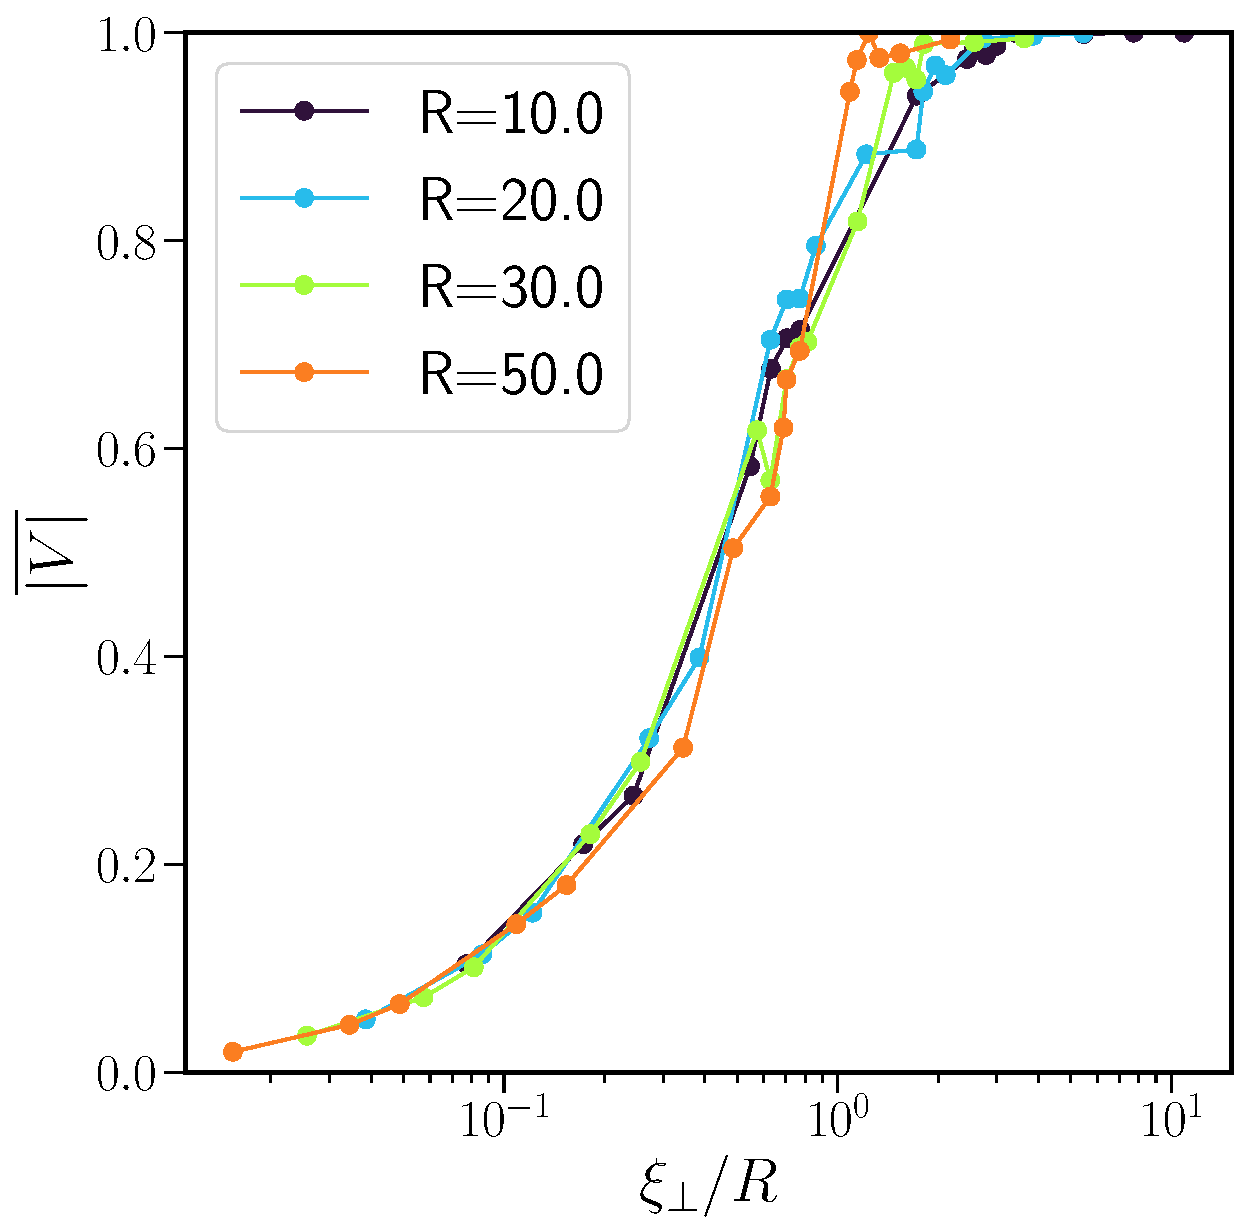
\includegraphics[width=\textwidth]{img/chiral/HAMLOD3_RAT40/abs_vlog_xdivide_Rx_sqrt_2.pdf}
        \end{minipage}
        \begin{minipage}{0.3\hsize}
            \text{(d)}
            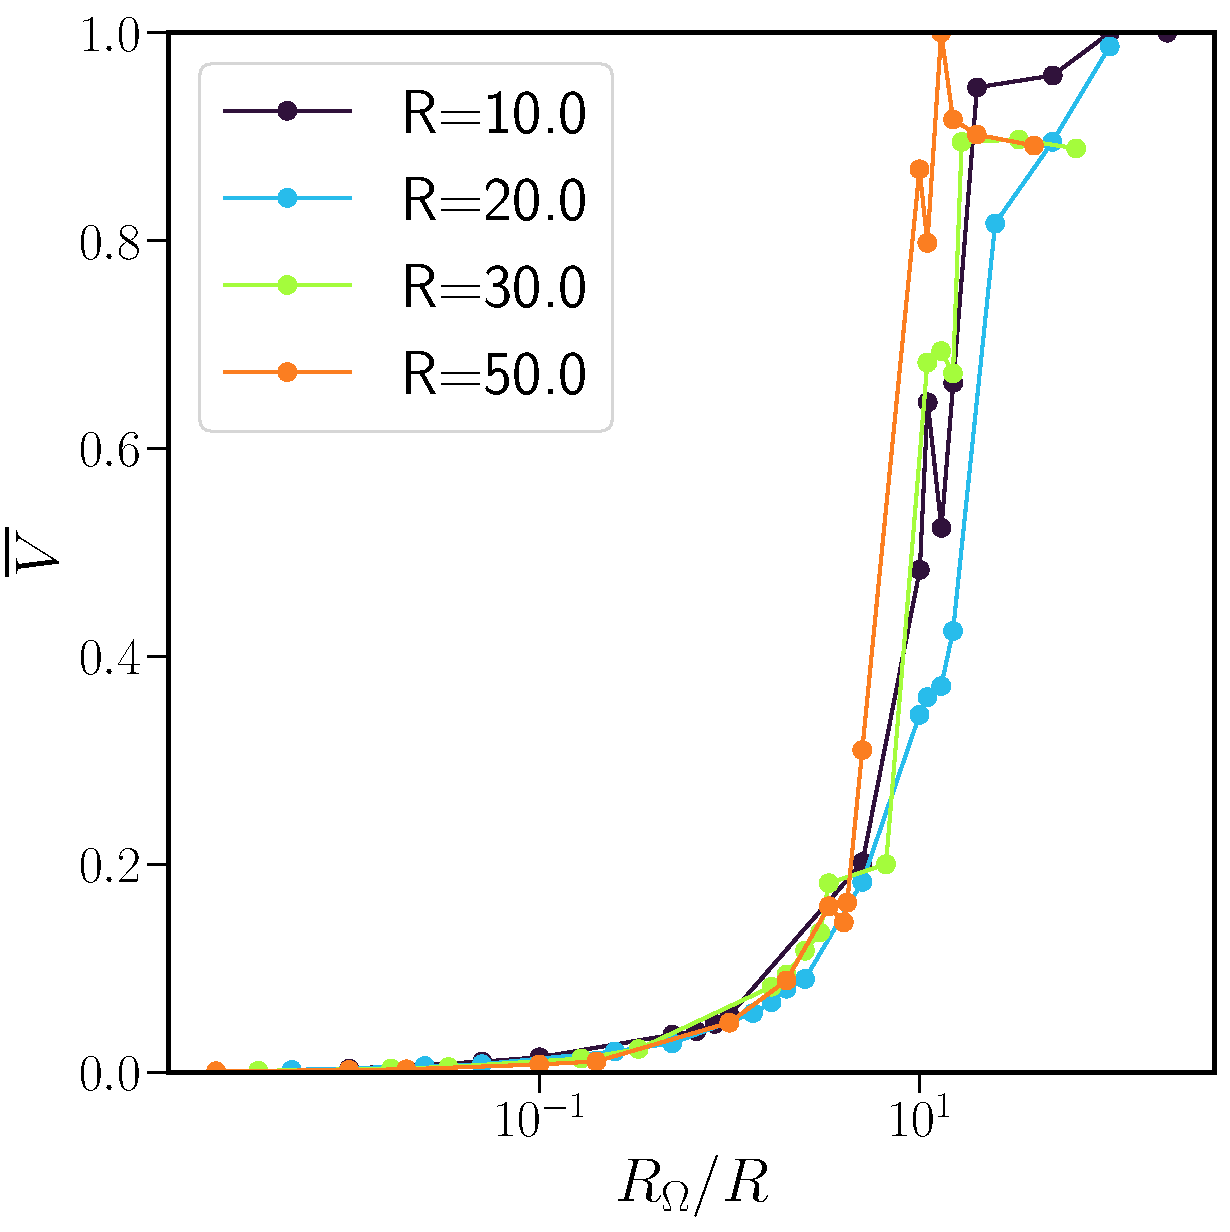
\includegraphics[width=\textwidth]{img/chiral/HAMLOD3_RAT40/sumvlog_xdivide_R.pdf}
        \end{minipage}\\
        \begin{minipage}{0.6\hsize}
            \text{(e)}
            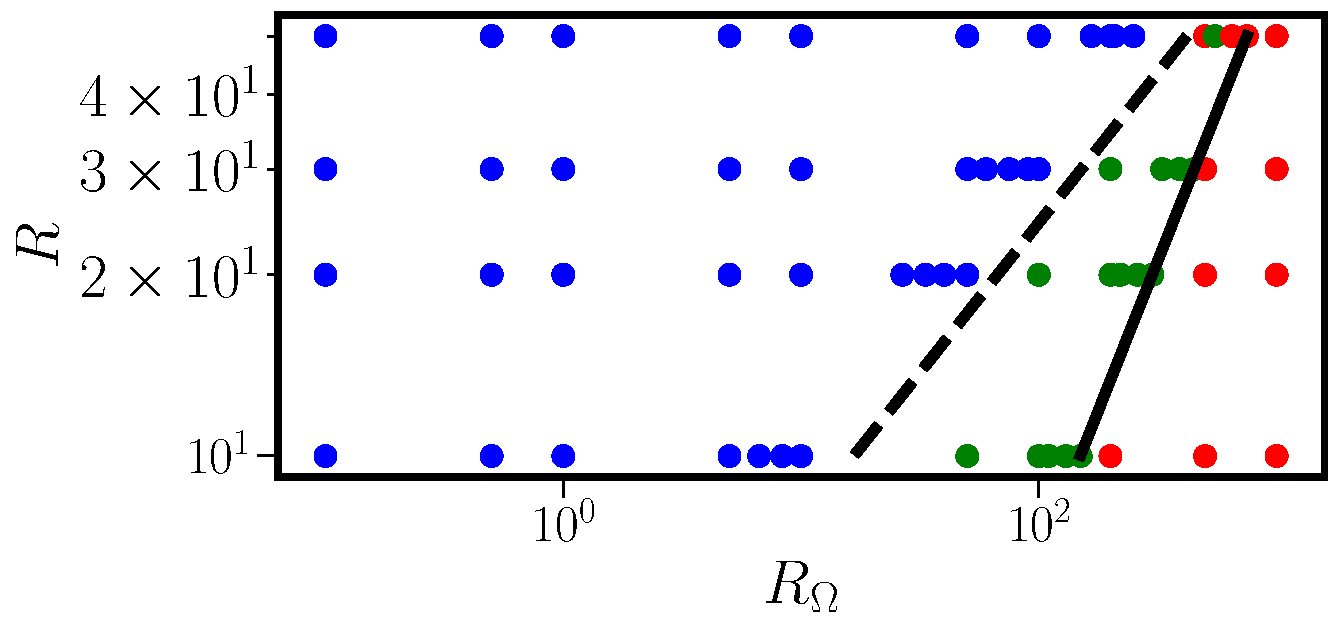
\includegraphics[width=\textwidth]{img/chiral/HAMLOD3_RAT40_diagram.pdf}
        \end{minipage}
    \end{tabular}
    \caption[Four sample images]
    {
        $V$の時間平均の値。(a)、(c)は$V$の絶対値の平均値、(b)、(d)は$V$の平均値のグラフ。
        横軸は$R_{\Omega}$で、横軸のみ対数軸である。
        (c)は横軸を$\xi_\bot/R \propto R_\Omega^{1/2}/R$\cite{kurodaLongrangeTranslationalOrder2024}で、
        (d)は横軸を$R_\Omega/R$でそれぞれスケールしてある。\\
        (e)は$\langle |\bar{V}| \rangle$と$\langle \bar{V} \rangle$の値を元にした相図。
        横軸は$R_\Omega$、縦軸は$R$であり、両軸は対数軸。
        $\langle |\bar{V}| \rangle<0.8$かつ$\langle \bar{V} \rangle<0.8$の点を青色、
        $\langle |\bar{V}| \rangle>0.8$かつ$\langle \bar{V} \rangle<0.8$の点を緑色、
        $\langle |\bar{V}| \rangle>0.8$かつ$\langle \bar{V} \rangle>0.8$の点を赤色にしてプロットしている。
        図中の点線は$R=\xi_\bot\propto R_\Omega^{1/2}$を、実線は$R\propto R_\Omega$を
        表す。
    }
    \label{fig:vabs_vave_state}
\end{figure}
振動相と定流相の間の遷移はRef \cite{capriniSelfrevertingVorticesChiral2024}と同様に、
1つの粒子が幅が$1\sigma$のリングの中に閉じ込められている状態を考えることで理解できる。
$R_\Omega$が半径$R$よりも大きい時、粒子の自己推進の方向はリングの接線方向と常に一定の角度を
なしている。しかし$R_\Omega$が半径$R$よりも小さい時、粒子がリングを一周するよりも早く自己推進の方向が
一周するため、粒子は進行方向を反転し、結果周期的な運動をする。\\%TODO:持っと簡単な説明
\figref{fig:vabs_vave_state}(e)はこれらの結果を元に描いた相図である。縦軸は$R$、横軸は$R_\Omega$で、
両方の軸は対数である。$\langle |\bar{V}| \rangle<0.8$かつ$\langle \bar{V} \rangle<0.8$の点を青色、
$\langle |\bar{V}| \rangle>0.8$かつ$\langle \bar{V} \rangle<0.8$の点を緑色、
$\langle |\bar{V}| \rangle>0.8$かつ$\langle \bar{V} \rangle>0.8$の点を赤色にしてプロットした。
図中の点線は$R=\xi_\bot\propto R_\Omega^{1/2}$を、実線は$R\propto R_\Omega$を表す。
この図からも分かるように、$R=\xi_\bot\propto R_\Omega^{1/2}$の線で乱雑相と振動相が、
$R\propto R_\Omega$の線で振動相と定流相が分けられることがわかる。
%周期(時間依存性)
%全体うず(相図)
%ふくうず
\subsection{部分}%TODO:タイトルを治す
続いて、円の中に発生する渦について調べる。

\begin{figure}[htbp]
    \centering
    \begin{tabular}{c}
        \begin{minipage}{0.24\hsize}
            \text{(a)}
            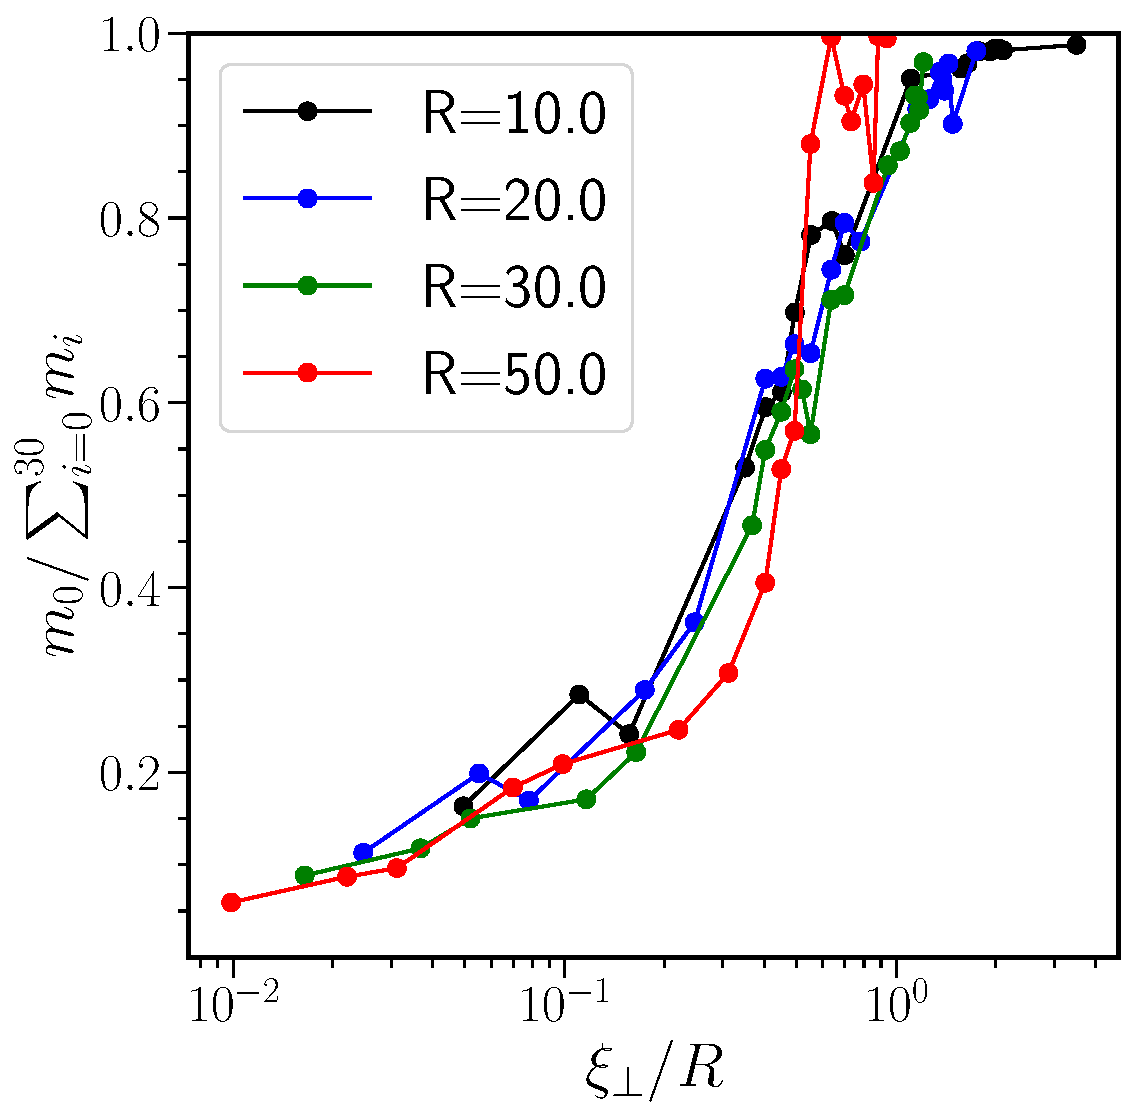
\includegraphics[width=\textwidth]{img/chiral/HAMLOD3MORE_RAT40/vel_modes_0log_xdivide_Rx_sqrt_2.pdf}
        \end{minipage}
        \begin{minipage}{0.24\hsize}
            \text{(b)}
            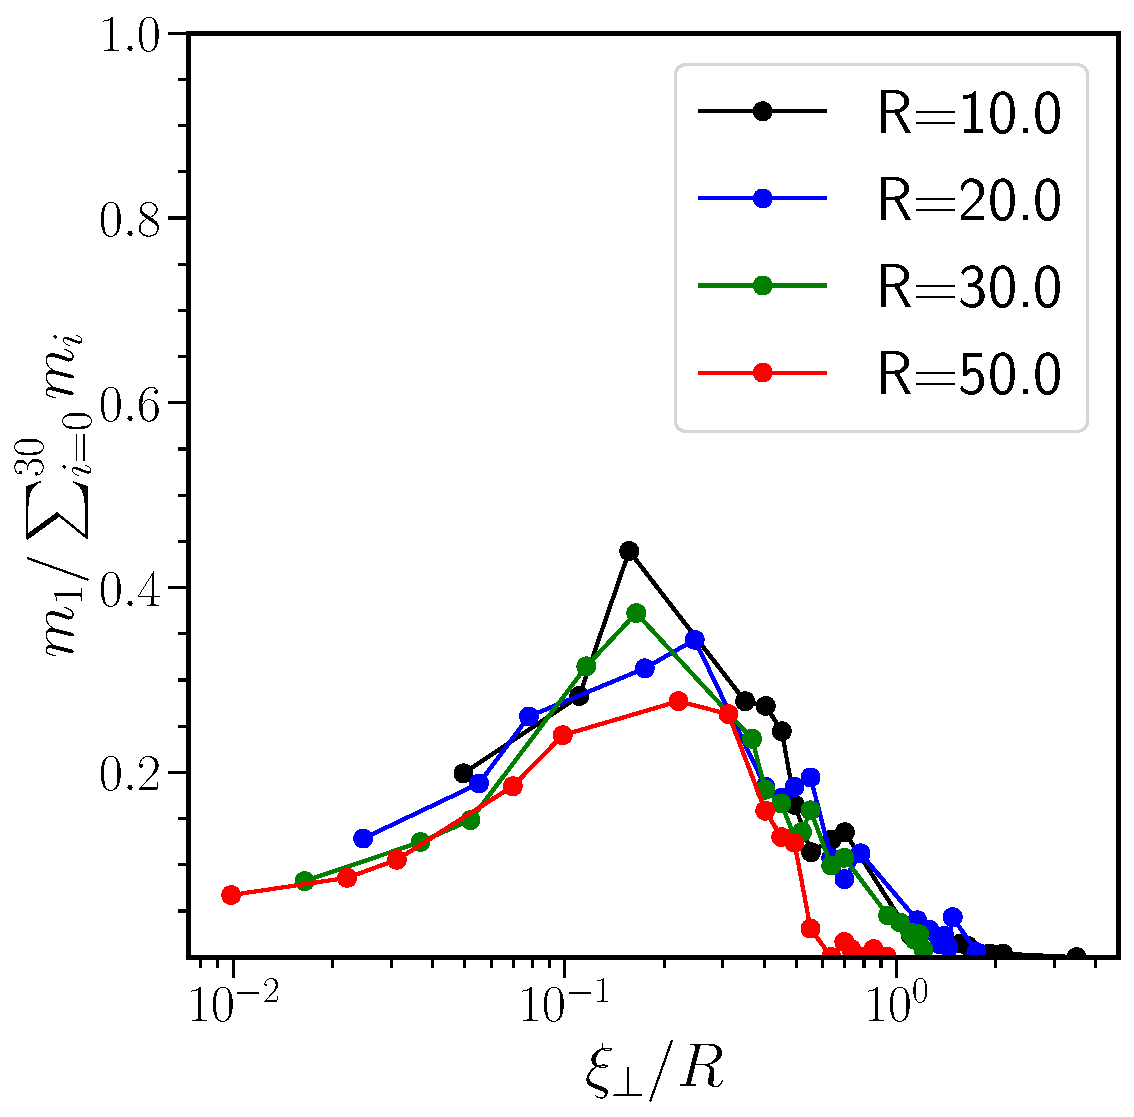
\includegraphics[width=\textwidth]{img/chiral/HAMLOD3MORE_RAT40/vel_modes_1log_xdivide_Rx_sqrt_2.pdf}
        \end{minipage}
        \begin{minipage}{0.24\hsize}
            \text{(c)}
            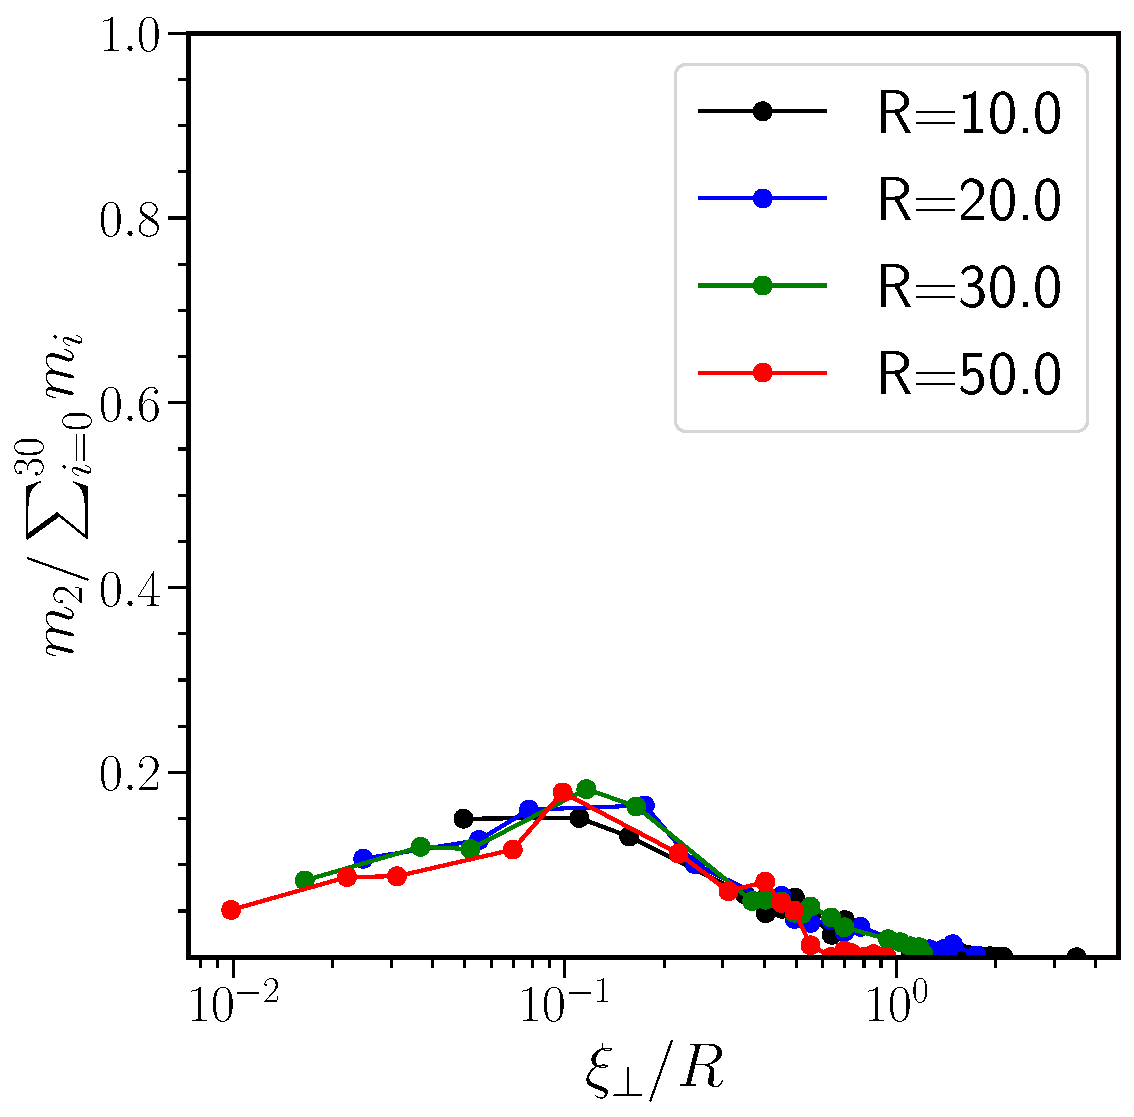
\includegraphics[width=\textwidth]{img/chiral/HAMLOD3MORE_RAT40/vel_modes_2log_xdivide_Rx_sqrt_2.pdf}
        \end{minipage}
        \begin{minipage}{0.24\hsize}
            \text{(d)}
            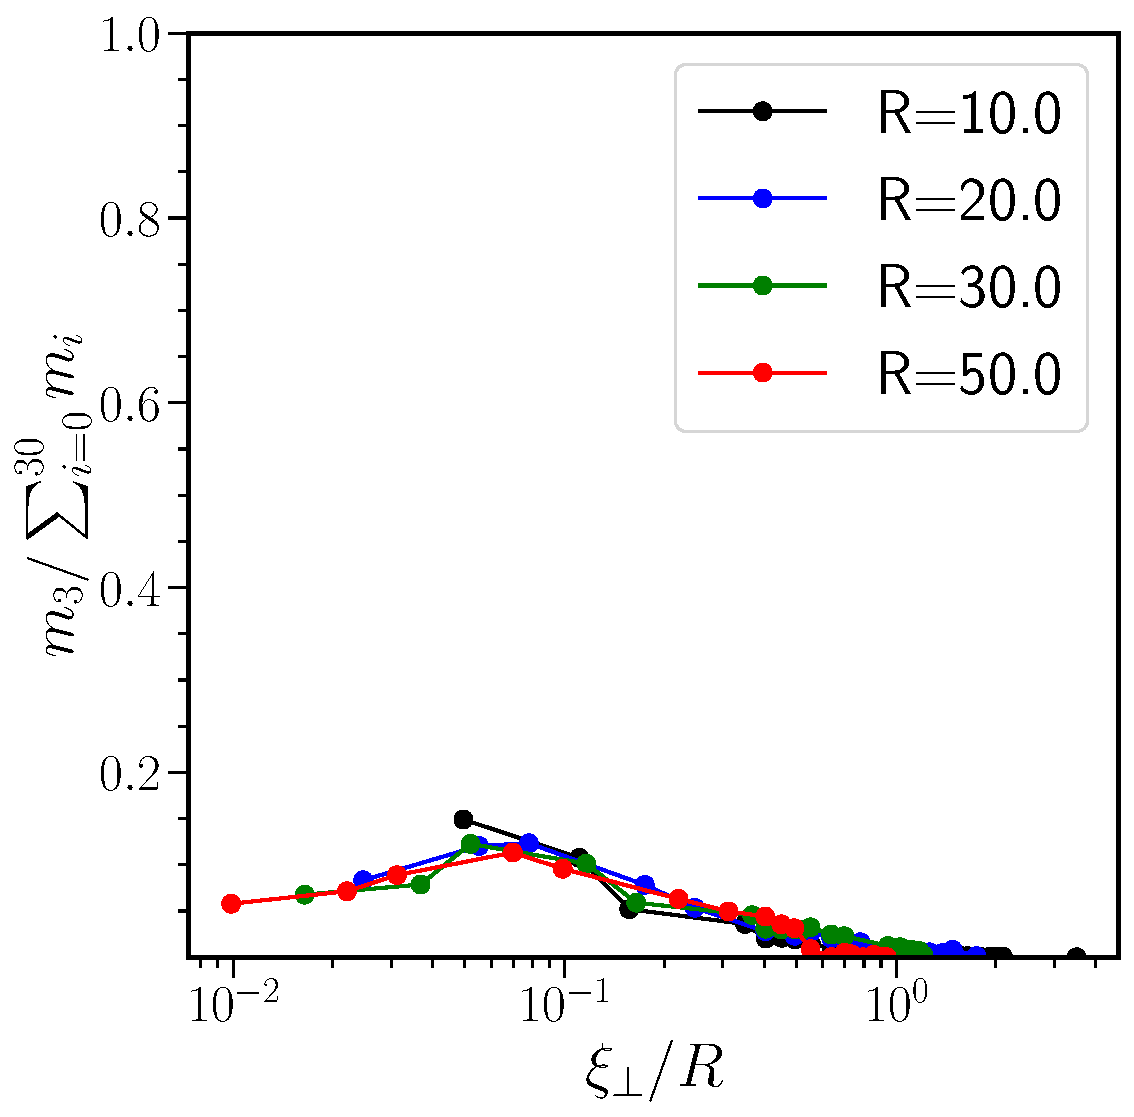
\includegraphics[width=\textwidth]{img/chiral/HAMLOD3MORE_RAT40/vel_modes_3log_xdivide_Rx_sqrt_2.pdf}
        \end{minipage}
    \end{tabular}
    \caption[Vel_modes]
    {
        角運動量成分の運動量。(a) $\langle m_0 \rangle$ (b) $\langle m_1 \rangle$ (c) $\langle m_2 \rangle$ (d) $\langle m_3 \rangle$。
        ただし、各パラメータにおける粒子速度の違いによる影響を避けるため、$n=0$から$n=30$までのモードの和で割ることで規格化している。
        横軸は相関長$\xi_\bot/R$\cite{kurodaLongrangeTranslationalOrder2024}でスケールしており、対数軸を使っている。
    }
    \label{fig:chiral_vel_modes}
\end{figure}

\ifSubfilesClassLoaded{
    \printbibliography[title=参考文献]
    % \printbibliography[title=参考文献]

    }{}
\end{document}
